\documentclass[pdftex,12pt,a4paper]{report}
\usepackage[pdftex]{graphicx}
\usepackage[francais]{babel} 
\usepackage[utf8]{inputenc}
\usepackage[T1]{fontenc}
\usepackage[top=2cm, bottom=2cm, left=3cm, right=3cm]{geometry}
\usepackage{graphicx}
\usepackage[toc,page]{appendix} 
\usepackage{pdfpages}
\usepackage{color}
\usepackage{chngpage}
\usepackage{fancyhdr}
\usepackage{fancybox}
\usepackage[Sonny]{fncychap}
\usepackage{titlesec, blindtext, color}
\usepackage{lastpage}

\setcounter{tocdepth}{3}
\setcounter{secnumdepth}{3} 
\setlength{\headheight}{14pt}
\renewcommand\headrulewidth{1pt}
\fancyhead[L]{Signature}
\fancyhead[R]{EPITA}
\definecolor{gray75}{gray}{0.75}
\newcommand{\hsp}{\hspace{20pt}}

\titleformat{\chapter}[hang]{\Huge\bfseries}{\thechapter\hsp\textcolor{gray75}{|}\hsp}{0pt}{\Huge\bfseries}

\renewcommand\footrulewidth{1pt}
\fancyfoot[L]{Signature}
\fancyfoot[R]{Page \thepage/\pageref{LastPage}}

\newcommand{\HRule}{\rule{\linewidth}{0.5mm}}

\pagestyle{fancy}

\begin{document}
\begin{titlepage}
\begin{center}
\textsc{\LARGE Signature}\\[1.5cm]

% Title
\HRule \\[0.4cm]
{\huge \bfseries Signature}\\[0.4cm]
\HRule \\[1.5cm]
\end{center}

% Author and supervisor
\begin{minipage}{0.4\textwidth}
	\begin{flushleft} \large
		\emph{Auteurs:}\\
			Victor \textsc{Degliame} \\
			Tanguy \textsc{Abel} \\
			Thibault \textsc{Lapassade} \\
			Florian \textsc{Thomassin} \\
	\end{flushleft}
\end{minipage}
\begin{minipage}{0.4\textwidth}
	\begin{flushright} \large
		\emph{Relecture:} \\
              Reda \textsc{Dehak}
	\end{flushright}
\end{minipage}
\end{titlepage}

\tableofcontents

\newpage

\chapter{Mise à l’échelle}

\newpage

\chapter{Dimension fractale}
La signature d'un individu est caractérisé par de multiple éléments qui ne sont pas discernable à l'œil nue.\\

Pour extraire ces caractéristiques, on peut calculer la dimension fractale qui d'après la définition permet d'obtenir une grandeur qui va traduire la façon dont un ensemble va remplir l'espace.\\

De plus, selon Mandelbrot, la dimension fractale permet de quantifier la complexité d'une courbe. C'est cette dernière qui nous intéressé pour la reconnaissance de signature.\\

Il existe de multiple définition de cette dimension, Hausdorff, homothétie, Minkowski-Bouligand. C'est cette dernière que nous utilisons, elle est aussi appelle "Box-Counting".\\

Cette technique est la plus utilisé et permet de mesurer numériquement la dimension fractale. Cela se fait via la formule suivante:

\vspace{0.3cm}
\begin{center}
\Ovalbox{$D_{box} = \lim\limits_{\epsilon \rightarrow 0}(\frac{log N(\epsilon)}{log N(1/\epsilon)})$ avec $N(\epsilon)$ nombre d'élément de diamètre $\epsilon$}
\end{center}
\vspace{0.3cm}

La méthode de Minkowski-Bouligand va recouvrir et créer un réseau de cube N fois sur la forme que l'on va analyser, N allant jusqu'à $+\infty$. En étudiant le comportement de ce réseau on va pouvoir calculer la dimension fractale.\\

\begin{figure}[!h]
	\begin{center}
		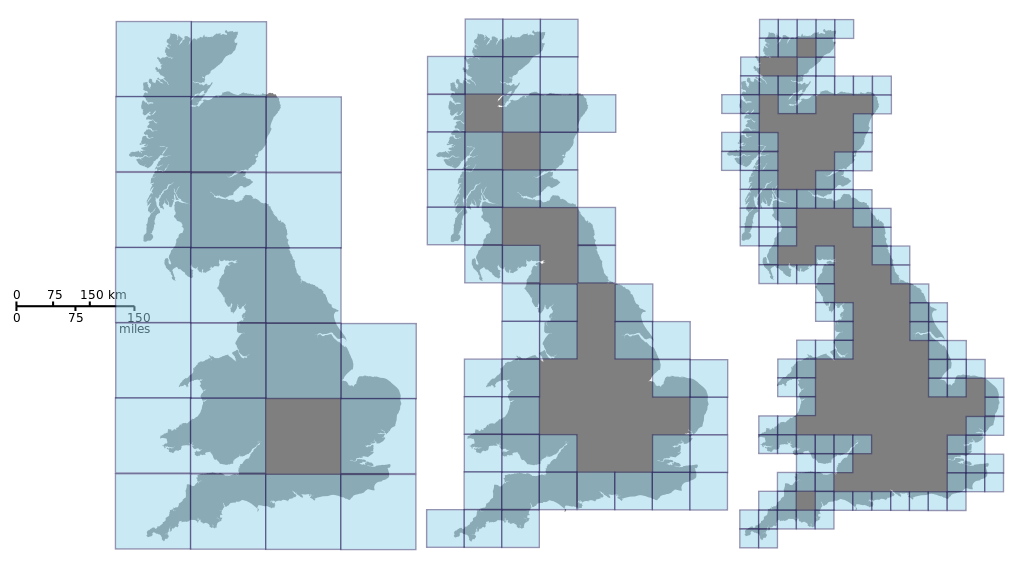
\includegraphics[scale=0.28]{images/Great_Britain_Box.png}
	\end{center}
\end{figure}

Grâce à cela nous pouvons donc avoir un facteur supplémentaire pour déterminer s'il y a contrefaçon ou non.

\newpage

\chapter{DTW}
C'est une méthode consistant à calculer la distance entre deux séries de valeurs. Elle est majoritairement utilisé dans le domaine de la reconnaissance de la parole mais dans notre cas, nous avons utilisé cette méthode pour calculer la distance entre les deux signatures que nous avions en entrée à partir de composantes extraites de ces images. \\

Nous avons préféré utiliser cette méthode plutôt que celle des HMM ou des GMM car d'après ce que nous avons pu trouvé lors de nos recherches, c'était celle-ci qui revenait le plus souvent comme la plus efficiente pour comparer deux signatures pouvant ne pas avoir le même nombre de points. La distance qui nous est renvoyé par notre DTW est partis prenante dans le choix que nous faisons ensuite pour dire si oui ou non les deux signatures appartiennent à la même personne ou non puisque nous avons remarqué empiriquement que cette distance est plus représentative de la personne qui a fait la signature que les autres caractéristiques que l'on pouvait extraire mais également parce que nos recherches nous ont conduit à confirmer cette information. Néanmoins, dans certains cas, cette distance n'est pas suffisante et il faut donc utiliser d'autres informations que celle-ci pour la comparaison.

\chapter{Décision}

\newpage

\end{document}